\section{\mc 背景}
約1世紀前にHans Bergerによって世界で初のヒトの脳活動計測の試みがなされた\cite{宮内1,宮内2,宮内3}。
以降、脳活動を計測するための測定装置が開発され、
特に近年は以下の応用を目指した脳信号の解析と解読に大きな関心が寄せられている。
\begin{itemize}
    \item 医療応用:脳信号は、認知症やてんかん発作のような様々な精神障害の診断、
    および治療のために活用されている\cite{精神疾患,認知症}。
    \item 生体認証:脳信号は偽造、盗聴が困難であることから、
    固体の識別のための普遍的な生体情報となりうる\cite{個人認証,ウェアラブル個人認証}。
    \item Brain Computer Interface(BCI):
    BCIは``direct neural interface''や``brain machine interface''とも表現され、
    外界と筋肉の動作無しに相互作用するためのインターフェースの役割を担う\cite{DNI}。
    特に研究初期におけるBCIは麻痺患者や障害のある患者の
    生活補助装置を制御するように設計された\cite{BCIbasic}。
    更に、近年は高度な精神的タスクを実行する健常者の支援や
    仮想空間での入力装置としての商用BCIを目指した研究も登場するに至っている\cite{VRBCI,VRBCIsv}。
    特に米国のFaceBook社が2017年4月に``Typing by Brain''プロジェクト(文字入力を行うBCIの開発)
    に取り組むことを発表し、産業界においても注目を浴びている。
\end{itemize}
本研究では医療の現場における患者の補助装置あるいはリハビリテーション装置としてのみならず、
産業応用への拡がりも見せているBCIに着目した。

\subsection{\mc 脳信号の計測}
BCIにおいて脳信号を計測する方法は、大きく分けて以下の3つがある\cite{BCImeasure}。
\begin{itemize}
    \item 侵襲式:脳へセンサを直接埋め込む方式
    \item 部分侵襲式:頭蓋骨の内部、脳の表面へセンサを埋め込む方式
    \item 非侵襲式:センサを頭蓋骨外部へ配置し、外科手術を必要としない方式
\end{itemize}
非侵襲式は外科手術の必要性がなく、
医療的な応用のみならず、商業利用に向けた更なる発展の可能性があるため
本研究では非侵襲式の計測方法に着目する。

BCIで用いられる非侵襲式の計測には以下のようなものがある\cite{脳を測る}。
\begin{itemize}
    \item functional Magnetic Resonance Imaging (fMRI):
    MRIによって脳活動時の血流によって生ずる磁場を測定する。
    この測定は、脳の神経細胞が活動中により多くの酸素を含む血流を必要とする
    という事実に基づいている。
    \item functional Near-Infrared Spectroscopy (fNIR):
    近赤外線電磁波を用いて、
    脳皮質の異なる部分における酸素化および脱酸素化ヘモグロビンの濃度を測定する。
    \item Magnetoencephalography (MEG):
    この方法は、高感度磁力計アレイを使用して、
    脳の神経活動によって生成される磁場を直接測定する。
    MEGを利用する大きな利点は、
    頭蓋骨や他の組織は磁場に対してほとんど透明であるため、
    減衰や歪みが生じないことが挙げられる。
    \item Electroencephalography (EEG):
    この方法では頭皮上にいくつかの小さな電極を配置し、
    脳全体の神経アセンブリによって生成された電場を測定する。
\end{itemize}
これらの方法の中で、fMRIおよびMEGは、fNIRおよびEEGと比較して比較的高い空間分解能を提供する\cite{脳を測る}。
しかし、fMRI(図\ref{fig:fMRI})及びMEG(図\ref{fig:MEG})
は非常に高価な装置である上に大型機器であるため、
BCIアプリケーションで必要とされるような要件を満たすとは言い難い。
一方でfNIRはポータブルであるが、
脳活動から数秒程度の遅れで測定が行われるという欠点を有する\cite{脳を測る}。
\begin{figure}
    \begin{center}
    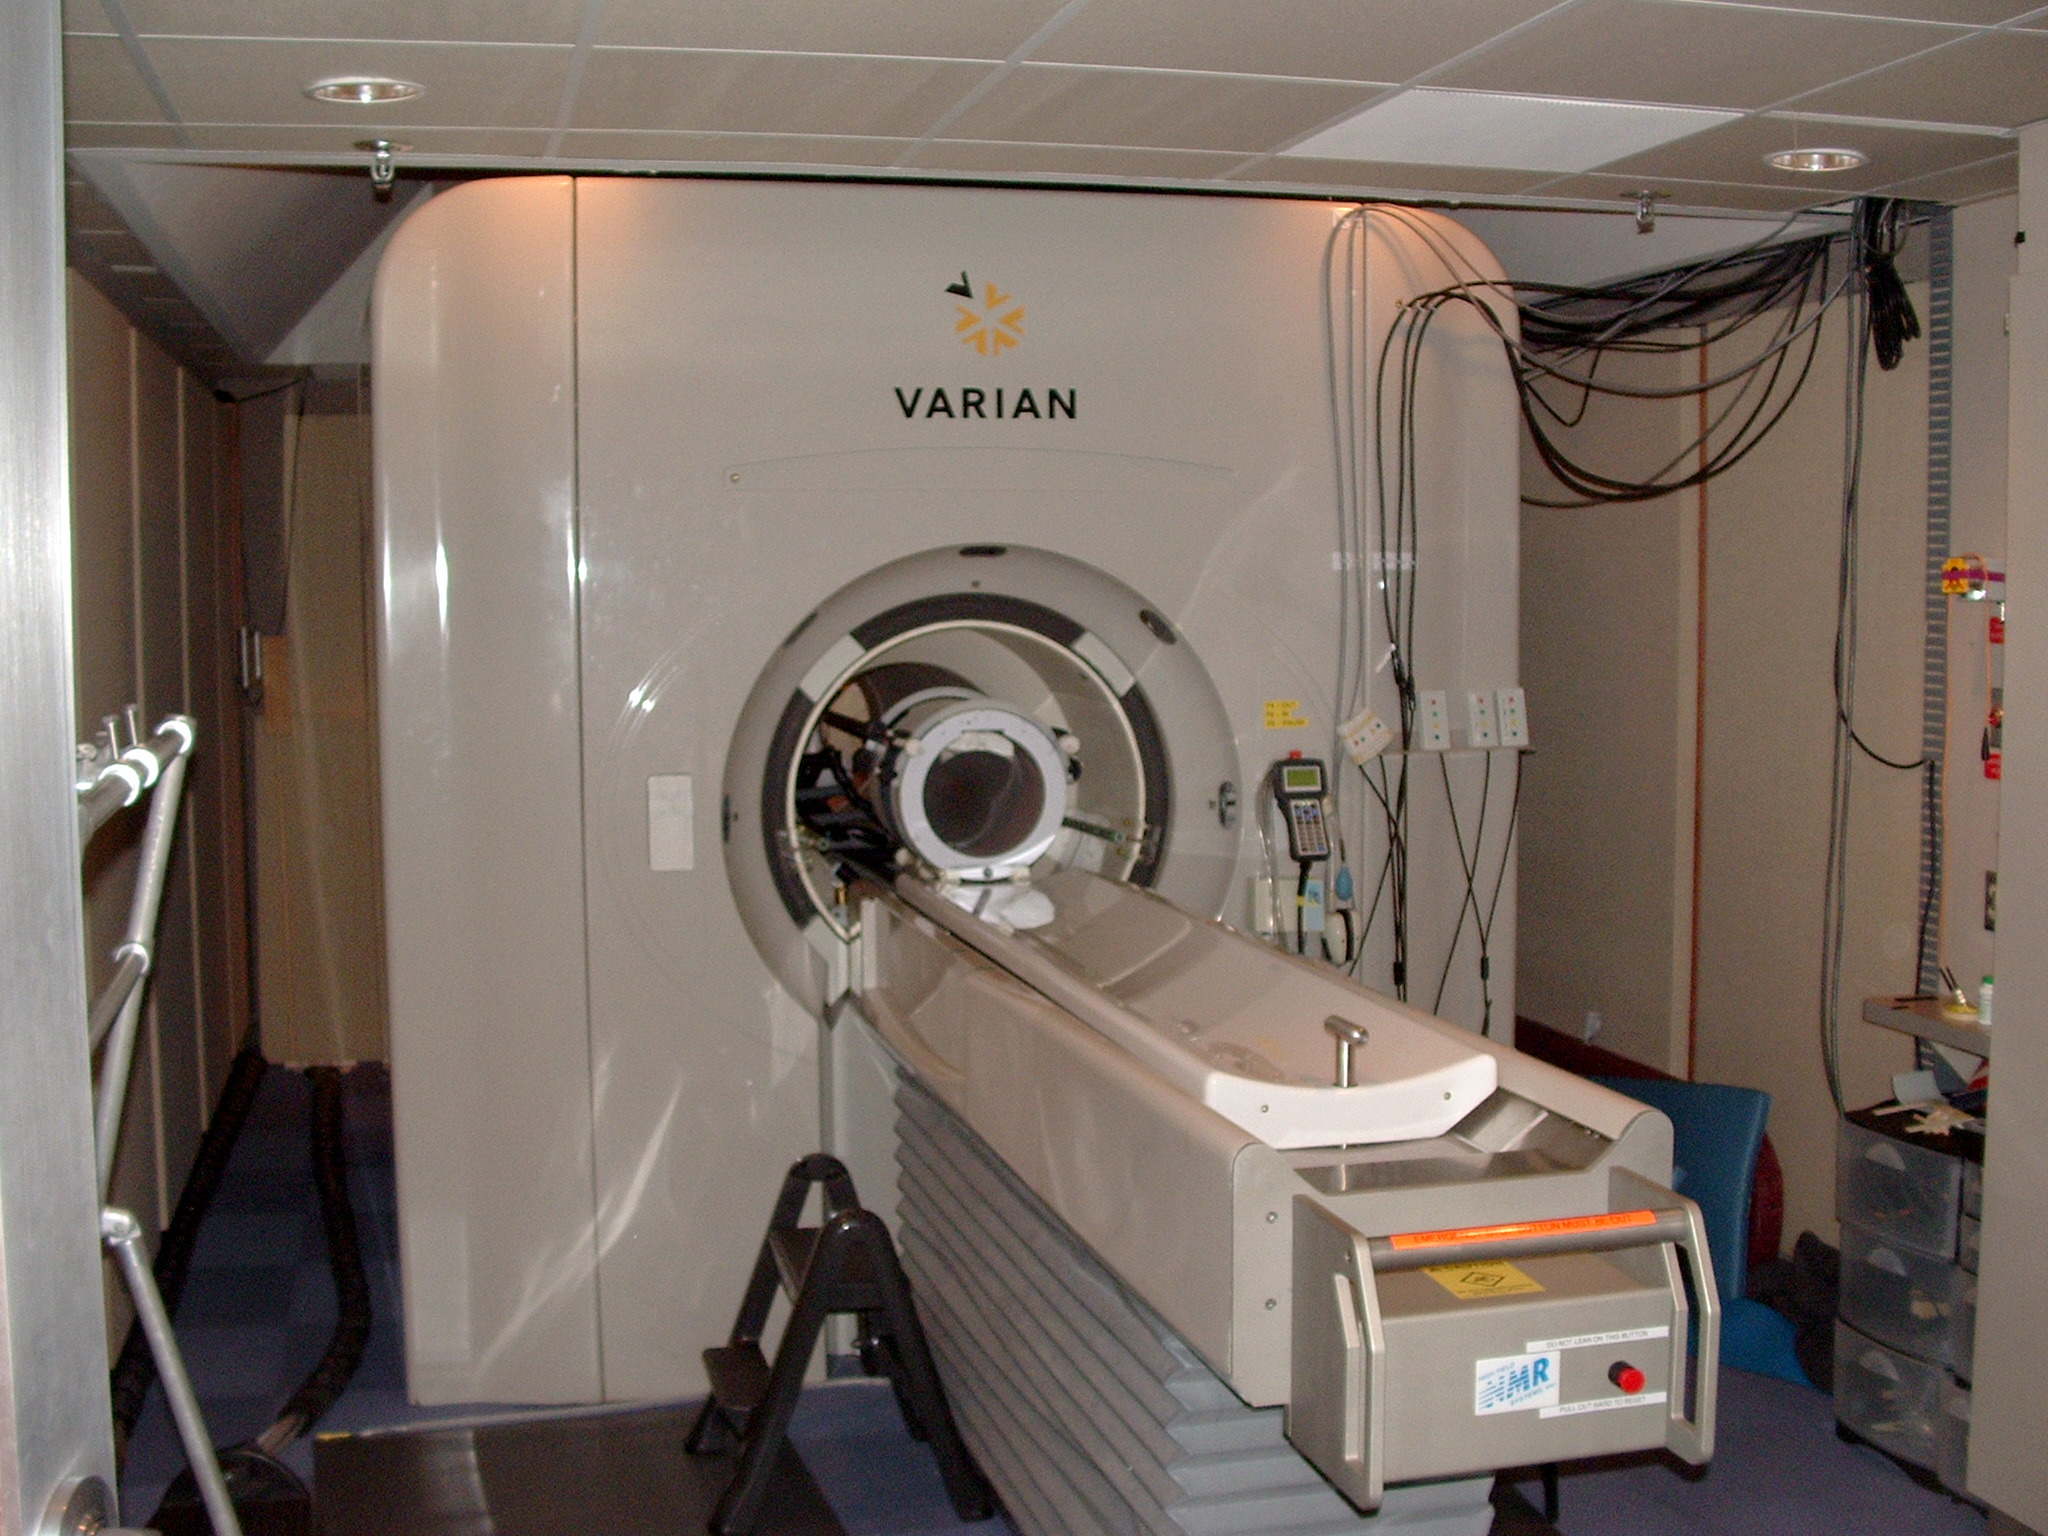
\includegraphics[width=120mm]{images/fMRI.jpg}
    \end{center}
    \caption{fMRI}
    \label{fig:fMRI}
\end{figure}
\begin{figure}
    \begin{center}
    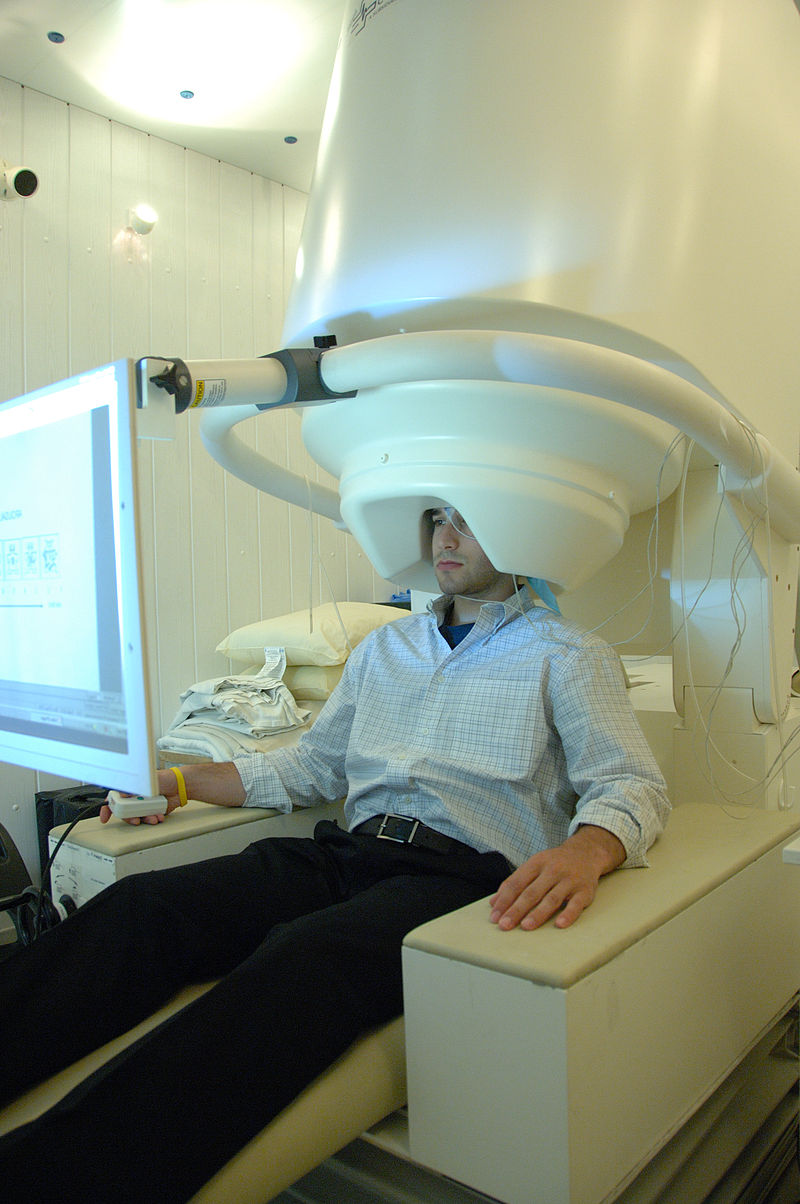
\includegraphics[width=70mm]{images/MEG.jpg}
    \end{center}
    \caption{MEG}
    \label{fig:MEG}
\end{figure}

\begin{figure}
    \begin{center}
    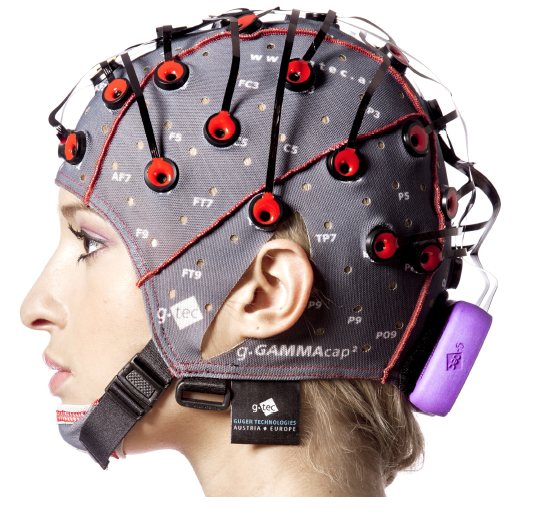
\includegraphics[width=60mm]{images/eeg.png}
    \end{center}
    \caption{EEGキャップ(ミユキ技研)}
    \label{fig:EEG}
\end{figure}
% \begin{figure}[t]
%     \begin{minipage}{0.5\hsize}
%         \begin{center}
%             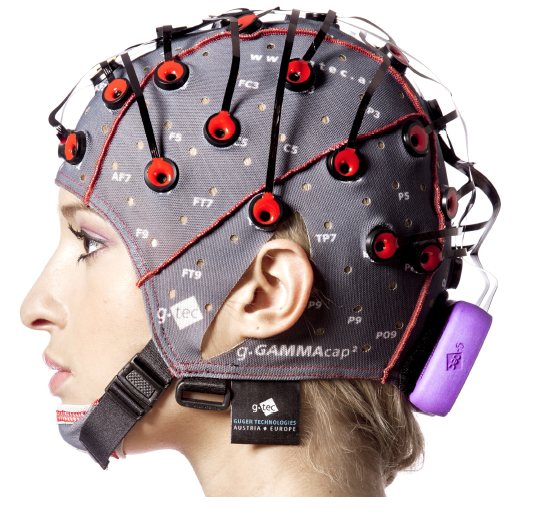
\includegraphics[width=60mm]{images/eeg.png}
%         \end{center}
%         \caption{fNIRキャップ(参照明記englishwiki)}
%         \label{fig:fNIR}
%     \end{minipage}
%     \begin{minipage}{0.5\hsize}
%         \begin{center}
%             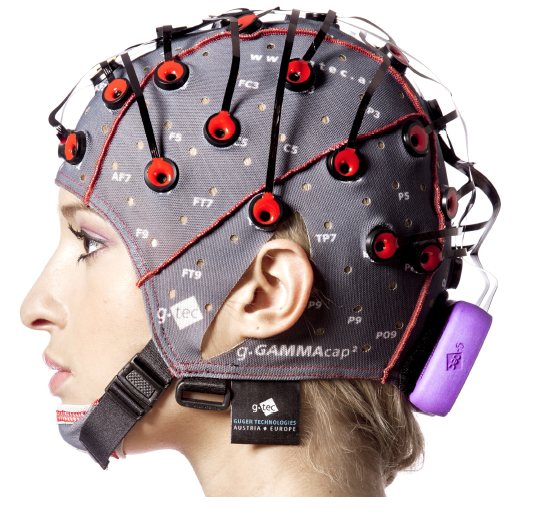
\includegraphics[width=60mm]{images/eeg.png}
%         \end{center}
%         \caption{EEGキャップ(ミユキ技研)}
%         \label{fig:EEG}
%     \end{minipage}
% \end{figure}

宮内氏の技術報告書\cite{脳を測る}によると、
EEGによる脳活動の計測に関して以下の記述がある(一部改変)。
\begin{quotation}
ヒトの脳活動計測によって獲得したいものは、精神活動・行動の生物学的基盤となる
脳の神経細胞(ニューロン)の電気的活動だが、
個々のニューロンの活動を非侵襲的に計測する事は不可能である。
しかし、ニューロンの活動に伴って様々な生理現象が生ずる。
まずニューロンが電気的な活動(一次信号)を行うためにはエネルギーを必要とし、
糖の分解のための代謝活動(二次信号)が生ずる。
酸素と糖は脳にはほとんど貯蔵されていないため、
代謝活動に伴ってエネルギーを必要としている脳の部位に関して、局所脳血流(三次信号)が増大する。
EEGやMEGは脳の電気的な活動である一次信号を計測しており、
fMRIやNIRSは血流に関する三次信号を計測している(図\ref{fig:信号フロー}\cite{脳を測る})。
\end{quotation}
\begin{figure}
    \centering
    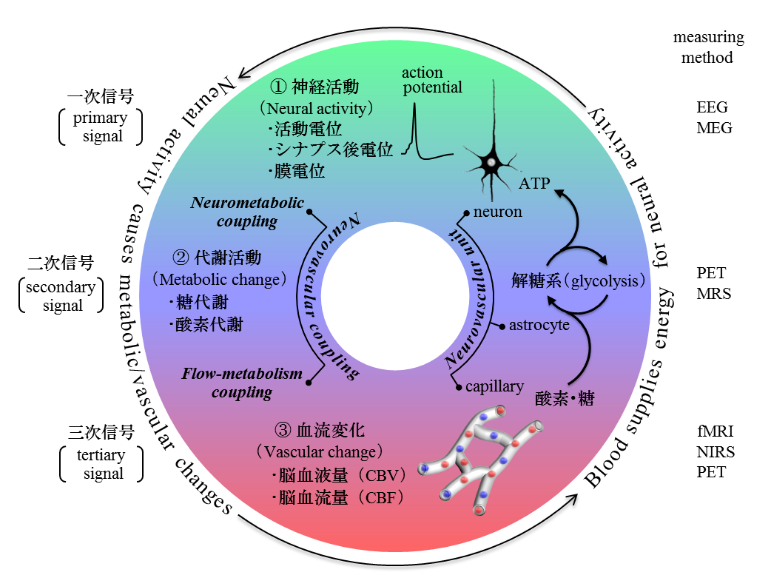
\includegraphics[width=12cm]{images/signalflow.png}
    \caption{一次信号、二次信号、三次信号と計測方法の関係図\cite{脳を測る}}
    \label{fig:信号フロー}
\end{figure}
EEGは一次信号を計測したものであり
NIRSやfMRIに比べ脳活動に対する測定値の遅れは少ないことが利点となる。
この利点に加え、EEGの測定装置は比較的安価であるため本研究の焦点とする。

続いて同様に\cite{脳を測る}にはEEGの分解能に関して以下の記述がある。
\begin{quotation}
また非侵襲計測の中では最も時間分解能が高いとされる。
ここで時間分解能とは脳の同一の場所が短時間に二回活動した場合に、
それぞれを時間的に独立した脳活動として計測できる最短の時間間隔である。
一方で頭蓋骨や皮膚、毛髪などは電位にとっては透明ではないため空間分解能は低いとされる。
ここで空間分解能とは脳の異なる部位が同時に二箇所活動した場合に、それぞれを活動部位が異なる
独立した脳活動として計測できる最小の距離である。
ただし、通常の計測においては計測装置の空間分解能や時間分解能は測定対象には依存しないが、
脳活動計測の場合においては一般的に計測対象としている現象の時空間特性や脳活動の強さ、
あるいは発生源が皮膚表面であるか脳の深部であるかなどにも依存する。
\end{quotation}
時間分解能の高さはBCIをEEGに基づいて動作させる利点となるが、
空間分解能の低さは明らかな欠点となるため、何らかの対策が必要となる。

\subsection{{\rm EEG}\mc に基づく{\rm BCI}{\mc の概要}}
\subsubsection{\rm BCI\mc の動作原理}
BCIの動作を以下の流れに分けて説明する。
\begin{enumerate}
    \item 脳信号の獲得:センサによりアナログ信号を獲得しディジタル信号へ変換
    \item 信号の前処理:データの成形及びアーチファクトの除去
    \item 特徴量抽出:神経科学や統計に基づいた特徴量の選定
    \item 分類:特徴量から閾値に基づいて意図を分類
    \item 制御信号出力:分類結果に基づいて外部機器へ信号を出力
\end{enumerate}
BCIの種類に関わらず動作原理の根本は同様であるが、
スキームのどの段階に課題が生じるかは異なると考えられる。
侵襲式の場合は``1.脳信号の獲得''自体が外科手術を伴うために困難であり、
安全性やメンテナンス性に課題が生ずる。
一方で信号の発生源から直接信号を計測できるため、``2.信号の前処理''や``3.特徴抽出''
に対する課題は少ない。
``4.分類''に関しては神経科学に基づいた適切な処理が必要であるが、
既に肢体のキネマティックスを復元できるほどに精度が高い。
非侵襲式の場合は``1.脳信号の獲得''は気軽に実施できるが、信号源とセンサの間には
各組織の細胞や頭蓋骨、頭皮や毛髪などがあるために測定値にはノイズが混入していると考えられる。
従って``2.信号の前処理''を行い脳信号を適切に取り出し、更に人間の意図を復元するような優れた``3.特徴量抽出''を行い
精度の高い``4.分類''を行うことが課題となる(図\ref{fig:BCIsystem})。

\begin{figure}[tb]
    \centering
    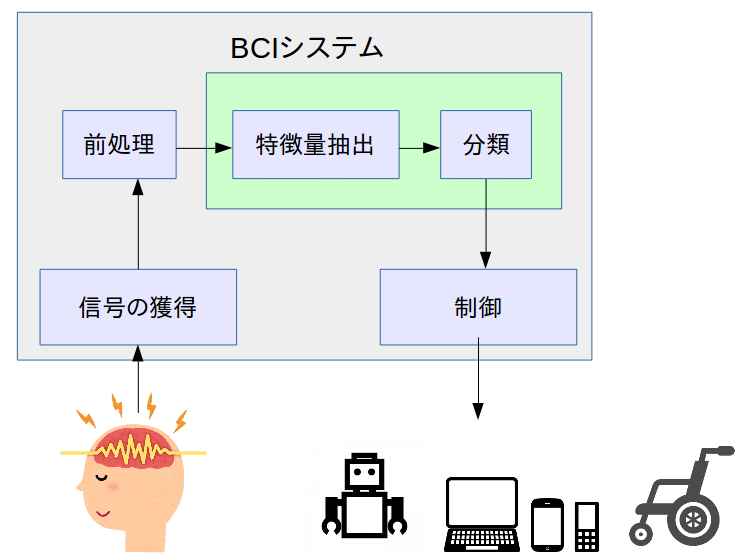
\includegraphics[width=13cm]{images/BCIsystem.png}
    \caption{BCIの動作スキーム}
    \label{fig:BCIsystem}
\end{figure}

またEEGに基づくBCIシステムに関しても、
着目するEEGの種類に応じて以下の二種に大別することができる。
\subsubsection{{\mc 誘発型}\rm BCI}
外部刺激によって誘発されるタイプのBCIを本論文では誘発型BCIとまとめて表記する。
例として、ユーザがBCIシステムを使用してマウスカーソルを動作させたいとする。 
この時、異なる周波数で点滅する複数の光源をユーザに提示することで、
注視した光源に応じた誘発電位を生成させることができる\cite{SSVEP}。
結果として、光源を見たユーザの脳信号を分析することでマウスカーソルの動作方向を決定することが可能である。
% このタイプのBCIは通常、SSVEP型BCIと呼ばれる。

誘発電位を用いたBCIシステムは非常に正確であるが、
ユーザは常に刺激に直面するため、長期的な使用には向いていないと考えられる。
また、BCIシステム自体が刺激装置などの外部機器を必要とする。
\subsubsection{\mc 自発型 \rm BCI}
一方で外部刺激に依らないEEGを用いて動作するBCIを自発型BCIと呼ぶ。
自発型BCIの中でも特に、特定の身体部位の動作を想像することで動作する運動想起型BCIに注目する。
運動想起型BCIの簡単な例を示すために、ユーザがBCIシステムを使用してマウスカーソルを動作させる例を見る。
この時、マウスカーソルを左に動かしたい場合は左手の運動を想起し、マウスカーソルを右に動かしたい場合は右手の運動を想起する。
また、下に動かしたい場合は左足、上に動かしたい場合は右足、
というように想起する身体部位に応じて外部機器への制御信号を対応させることが可能である。
同様の応用方法が車いすなどにも適用できる。

運動想起型BCIを使う利点の1つは、運動想起によって生成されたEEG信号は、
物体の想像、あるいは抽象的な概念を想像する他の精神的イメージのタスクと比較して一貫性がある点である。
一般に、運動想起によって活性化される神経は、運動を実際に実行する場合と同様であるとされる\cite{運動想起}。
本研究では運動想起型BCIに焦点を当てる。
これまでのBCIの分類について図\ref{fig:BCIclass}に示す。

\begin{figure}[tb]
    \centering
    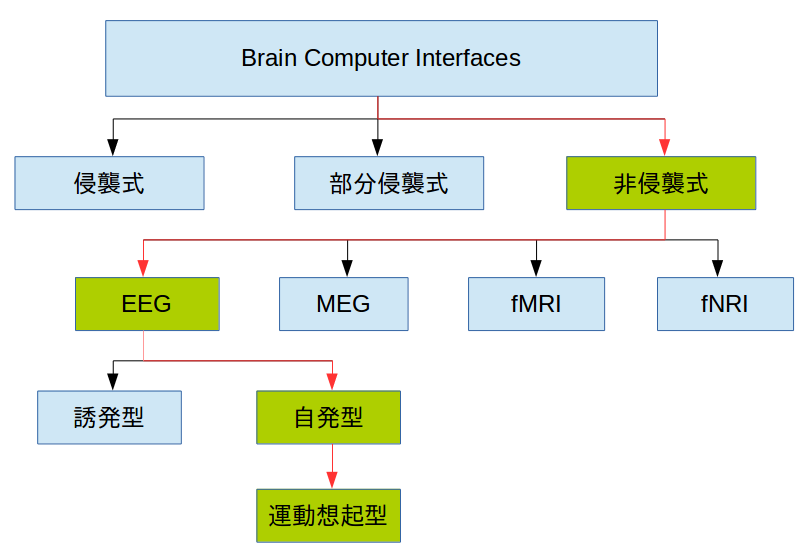
\includegraphics[width=13cm]{images/BCIclass.png}
    \caption{BCIの分類と本研究の焦点}
    \label{fig:BCIclass}
\end{figure}


\subsection{\mc 運動想起型\rm BCI\mc 周辺の研究}
運動想起時には運動野付近で特定の周波数帯域において活動電位が減少する
事象関連脱同期(Event Related Desynchronization : ERD)と、
ERDの発生後に活動電位が増大する事象関連同期(Event Related Synchronization : ERS)が知られている\cite{ERDとERS}。
ERDに関しては特に研究が盛んで、\cite{ERDリハビリ}では感覚情報として電気刺激を与えた場合のERDへの影響が調べられており、
また、運動想起時における脳活動を被験者にフィードバックすることでERDの出現に差異が生ずることが\cite{運動フィードバック}
にて調べられるなどの神経科学的な研究がある。
また、ERDがBCIの動作スイッチの役割を担うほど再現性を有することが\cite{Beta波によるBCI}で調査されており、
EEGを用いた運動想起型BCIの代表的な特徴量となっている。
ERDを特徴量に使う場合には特定の頭皮領域のEEGに対して短時間フーリエ変換を用いる方法
\cite{プリミティブERD}やウェーブレット変換を用いる方法\cite{waveletFSVM}が提案されている。
これらの時間周波数解析に基づく方法では、EEGのある特定の周波数帯域に着目し、
パワースペクトル密度に閾値を設けて分類を行うことができる。
% しかし、EEGからERDを検知するための優れた手法は未だに開発されているとは言えない。
% 現在でも有望な時間周波数解析の手法についての検討が行われており、\cite{時間周波数解析の比較}では
% 短時間フーリエ変換、連続ウェーブレット変換、自己回帰モデルによる手法が比較されており。

また、人の随意運動の約0.5秒から1秒前に現れる運動準備電位も特徴量になると考えられている。
実動作以前に発生するという極めて特殊な現象であるため、
その特性からBCIが人の意志に対して優れた反応速度で動作することが期待され、
運動準備電位に基いて実肢体動作の分類を行う研究\cite{運動準備電位肢体}や、実指動作の分類を行う研究\cite{運動準備電位指}などがある。
実運動を行わなくとも運動準備電位が生ずるかを計測し\cite{運動準備電位想起}、実際にBCIへの適用を検討した例\cite{運動準備電位想起2}もある。

一方で特定のEEGの現象を直接獲得せずに運動想起型BCIを構築する手法も提案されており、
それらの多くが統計的信号処理や機械学習を活用したものである。
特にCommon Spatial Pattern(CSP)と呼ばれる手法は\cite{CSP1990}にて提案され、
2種類の脳波を区別するための空間フィルタとして有望であることが示唆された。
その後、過学習抑制のための正則化を導入したCSP\cite{正則化CSP}、
非線形な空間フィルタを獲得できるカーネル法を導入したCSP\cite{カーネルCSP}、
バンドパスフィルタと空間フィルタを同時に最適化するCSP\cite{csssp}などが提案された。
また、Filter Bank Common Spartial Pattern\cite{fbcsp}と呼ばれるCSPの
発展手法は、複数のバンドパスフィルタに対してそれぞれCSPを適用し、
各バンドパスフィルタとCSPを通過した複数の信号に対してLinear Discriminant Analysis(LDA)を用いて
特徴量の選定を再度行うことで、
頭皮領域と周波数領域を広くカバーした上で最適な特徴量を獲得可能にした。

% 現在、計算機の発展とBCIの産業応用への期待も相まって、
% EEGの現象として知られている既知の特徴量を人出で模索する手法から、
% 機械学習や統計的信号処理を活用した特徴量抽出手法と高度な分類器を組み合わせ
% 高い性能を発揮する手法の模索が行われている\cite{BCIの比較}。
